% !TEX root = main.tex
% 82 124 170 231
\subsection{Numerical Simulations}

In this section, we consider several situations that quadrotors in a platoon on an air highway may commonly encounter, and show via simulations the behaviors that emerge from the controllers we defined in Sections \ref{sec:liveness} and \ref{sec:safety}.

\subsubsection{Forming a Platoon}
We first consider the scenario in which some quadrotors are trying to merge onto an initially unoccupied highway. In order to do this, each quadrotor first checks for safety with respect to the other quadrotors, and uses the safety controller if necessary, according to Section \ref{sec:safety}. Otherwise, the quadrotor uses the liveness controller described in Section \ref{sec:liveness}. 

For the simulation example, the highway is specified by the line $p_y = 0.5p_x$, the point of entry on the highway is chosen to be $(\bar{p}_x, \bar{p}_y) = (4,2)$, and the velocity on the highway is chosen to be ($\bar{v}_x, \bar{v}_y) = \frac{\bar{v}}{\sqrt{0.5^2 + 1^2}} (0.5, 1)$. The velocity simply states that the quadrotors must travel at a speed $\bar{v}=3$ along the direction of the highway. This forms the target state $\bar{x}_H=(\bar{p}_x, \bar{v}_x, \bar{p}_y, \bar{v}_y)$, from which we define the target set $\mathcal{L}_H$ as in Section \ref{subsec:highway_merge}.

The first quadrotor that completes merging onto the empty highway creates a platoon and becomes its leader, while subsequent quadrotors form a platoon behind the leader in a pre-specified order according to the process described in Section \ref{subsec:platoon_merge}. Here, we choose $(\bar{p}_{x,r}, \bar{p}_{y,r})$ to be a distance $b$ behind the last quadrotor in the platoon, and $(\bar{v}_{x,r}, \bar{v}_{y,r}) = (0,0)$. This gives us the target set $\mathcal{L}_P$ that we need.

Figures \ref{fig:normal2} and \ref{fig:normal5} show the simulation results. Since the liveness reachable sets are in 4D and the safety reachable sets are in 6D, we compute and plot their 2D slices based on the quadrotors' velocities and relative velocities. 

Figure \ref{fig:normal2} illustrates the use of liveness and safety reachable sets using just two quadrotors to reduce visual clutter. The first quadrotor $Q_1$ (red disk) first travels in a straight line towards the highway merging point $\bar{x}$ (red circle) at $t=1.5$, because it is not yet in the liveness reachable set for merging onto the highway (red dotted boundary). When it is within the liveness reachable set boundary at $t=2.8$, it is ``locked-in" to the target state $\bar{x}_H$, and follows the optimal control in \eqref{eq:HJB_ctrl_syn} to $\bar{x}_H$. During the entire time, the $Q_1$ checks whether it may collide with $Q_2$ within a time horizon of $t_\text{external}$; we chose $t_\text{external}=3>t_\text{internal}$. However, since $Q_1$ never goes into the boundary of the safety reachable set (red dashed boundary), it uses the liveness controller the entire time.

After $Q_1$ has reached $\bar{x}_H$, it forms a platoon, becomes the platoon leader, and continues to travel along the highway. $Q_2$ (blue disk), at $t=7$, begins joining the platoon behind $Q_1$, by moving towards the target $\bar{x}_P$ relative to the position of $Q_1$. Note that $\bar{x}_P$ moves with $Q_1$ as $\bar{x}_P$ is defined in terms of the relative states of the two quadrotors. When $Q_2$ moves inside the liveness reachable set boundary for joining the platoon (blue dotted boundary), it is ``locked-in" to the target relative state $\bar{x}_P$, and begins following the optimal control in \eqref{eq:HJI_ctrl_syn} towards the target as long as it stays out of the safety reachable set (blue dashed boundary).

Figure \ref{fig:normal5} shows the behavior of all 5 quadrotors which eventually form a platoon and travel along the highway together. The liveness controllers allow the quadrotors to optimally and smoothly enter the highway and join platoons, while the safety controllers prevent collisions from occurring.

% 40 60 110 210
\begin{figure} \label{fig:fp}
    \centering
    \begin{subfigure}{0.23\textwidth} \label{subfig:fp_40}
        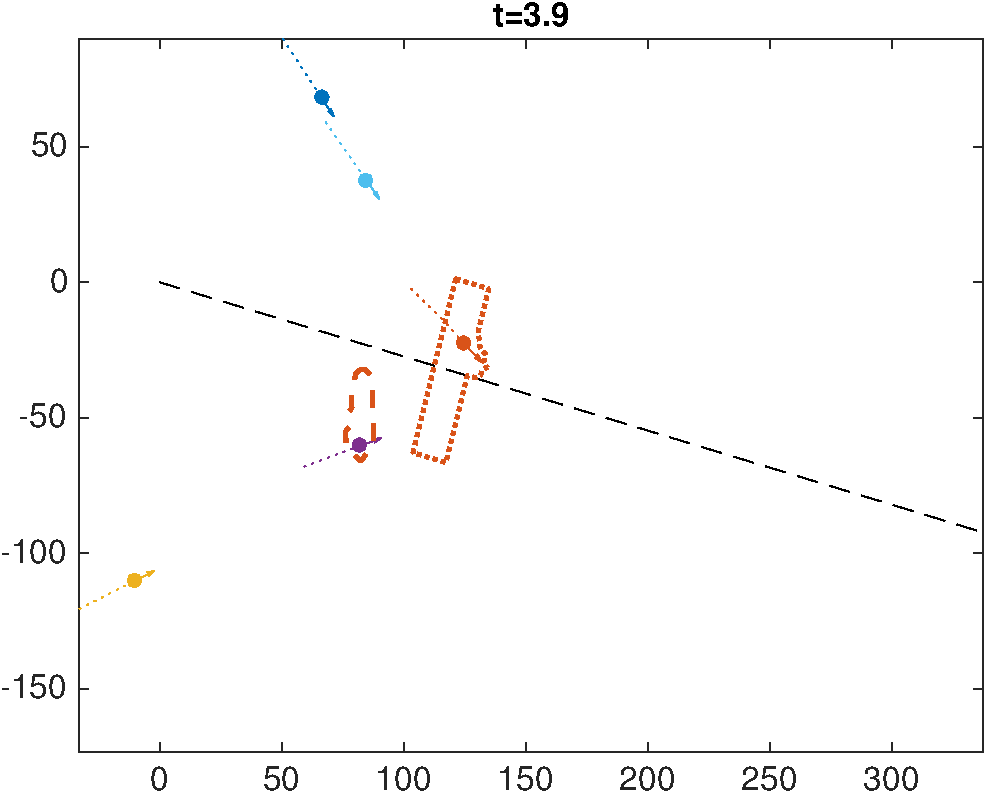
\includegraphics[width=\textwidth]{fig/fp_40}
        \caption{40}
    \end{subfigure}
    \begin{subfigure}{0.23\textwidth} \label{subfig:fp_60}
        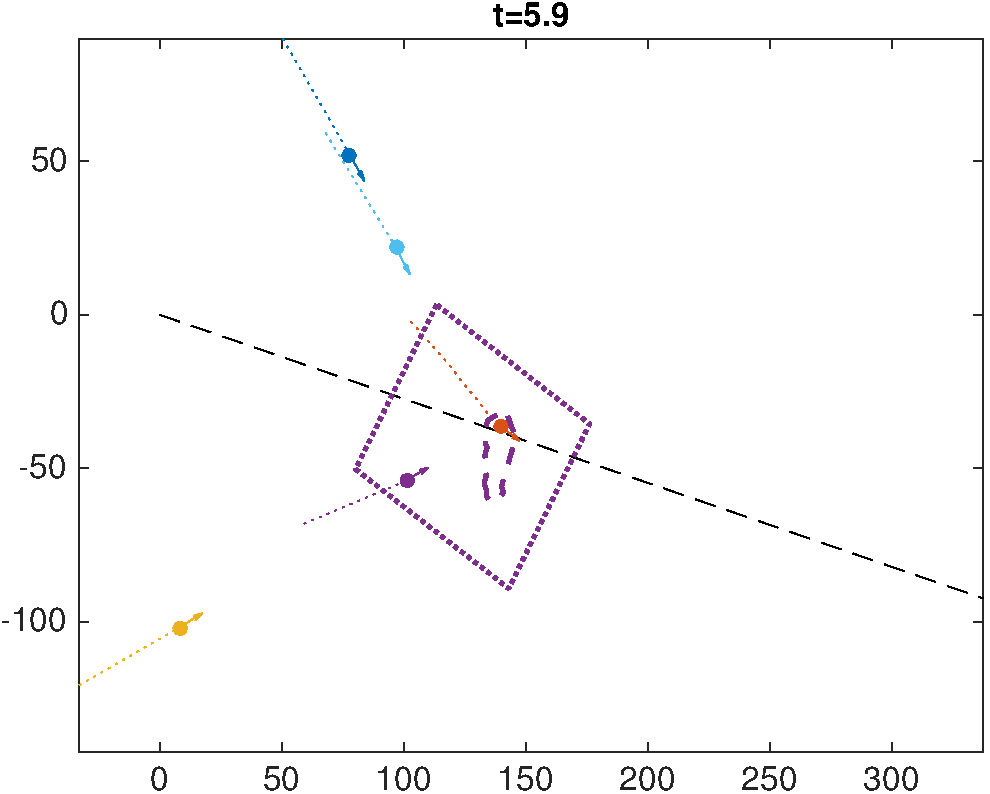
\includegraphics[width=\textwidth]{fig/fp_60}
        \caption{60}
    \end{subfigure}

    \begin{subfigure}{0.23\textwidth} \label{subfig:fp_110}
        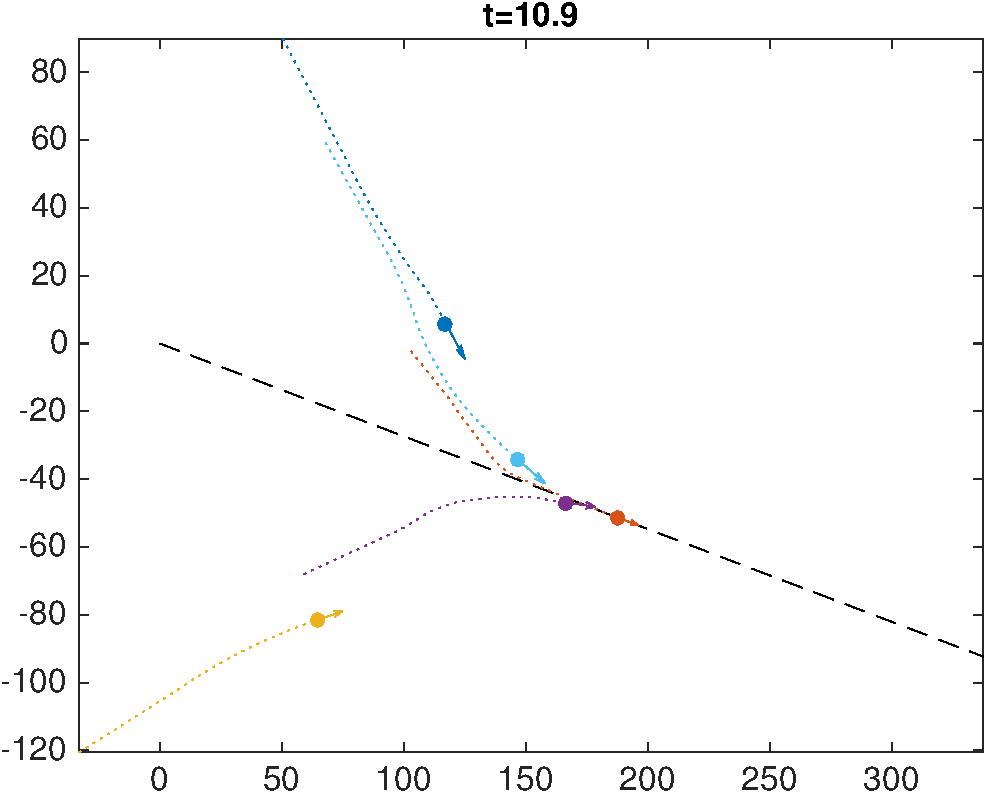
\includegraphics[width=\textwidth]{fig/fp_110}
        \caption{110}
    \end{subfigure}
    \begin{subfigure}{0.23\textwidth} \label{subfig:fp_210}
        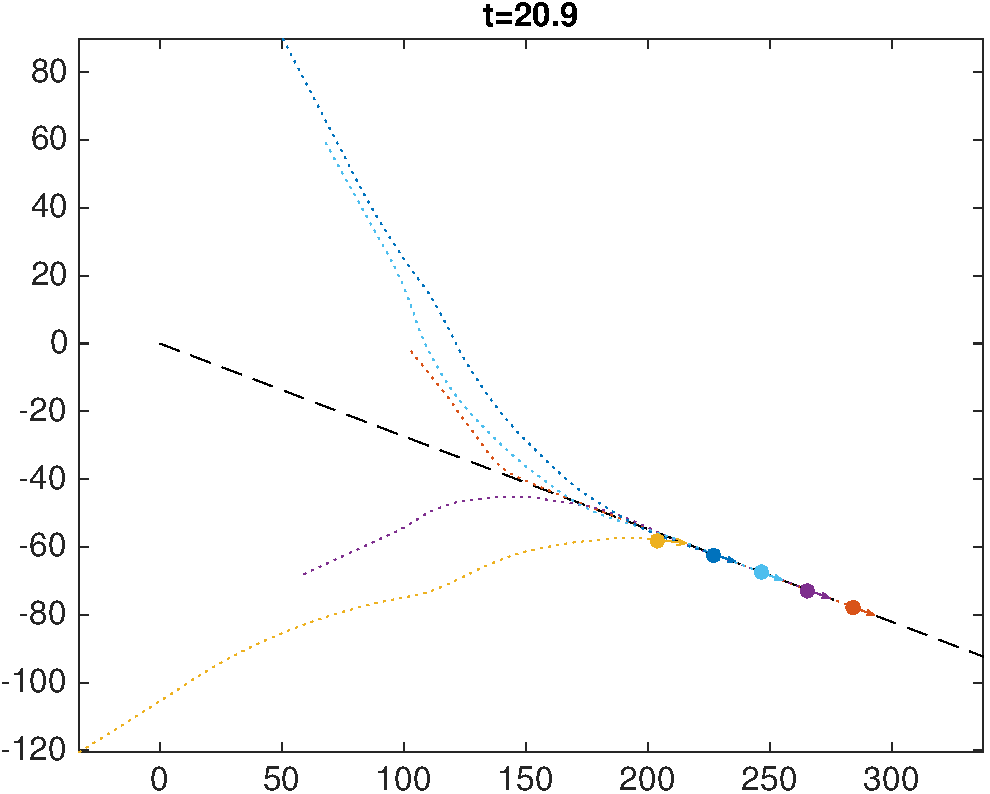
\includegraphics[width=\textwidth]{fig/fp_210}
        \caption{210}
    \end{subfigure}   
    \caption{form platoons}    
\end{figure}

\subsubsection{Intruder Vehicle}
We now consider the scenario in which a platoon of quadrotors encounters an intruder vehicle. To avoid collision, each quadrotor checks for safety with respect to the intruder and any quadrotor in front and behind in the platoon. If necessary, the quadrotor uses the safety controller, otherwise it uses the appropriate liveness controller, depending on whether it is a leader or follower.

Figure \ref{fig:intruder1} shows the simulation result. At $t=0$, a platoon of 4 quadrotors, $Q_{P_i},i=1,\ldots,4$ with $P_i = i$, travels along the highway defined by the line $p_y = p_x$. An intruder vehicle $Q_0$ (red disk) starts from position $(p_x, p_y) = (40,30)$ and heads toward bottom-left of the grid. As before, platoon members incur a safety breach if $V(-t_\text{internal},x_{P_i}-x_{P_j})\le 0$. However, with respect to $Q_0$, platoon members incur a safety breach if $V(-t_\text{external}, x_{P_i}-x_0) \le 0$ with $t_\text{external}>t_\text{internal}$. 

The platoon leader $Q_{P_1}$'s (black disk) safety is unaffected by the intruder, thus it simply follows its original path on the highway using the liveness controller described in Section \ref{sec:travel_hwy}. Followers $Q_{P_2}$ (blue disk), $Q_{P_3}$ (green disk) and $Q_{P_4}$ (pink disk), on the other hand, must use the safety controller in order to avoid collision with the intruder ($t=3.3,6.2$). This causes their paths to deviate off the highway. Once each quadrotor is safe relative to the intruder, they merge back onto the highway, join the original platoon and continue traveling along it ($t=12.4$).

Figure \ref{fig:intruder2} illustrates the use of safety reachable sets in this scenario using only $Q_{P_2}$ as an example. The safety reachable sets of $Q_{P_2}$ with respect to the intruder $Q_0$ (red dashed line), $Q_{P_1}$ (black dashed line) and $Q_{P_3}$ (green dashed line) are shown. With respect to $Q_0$, $Q_{P_2}$'s safety is considered to be breached if $V_S(-t_\text{external},x_{P_2}-x_0) \le 0$. To avoid possible collision with the intruder, $Q_{P_2}$ must remain outside the safety reachable set with respect to the intruder. The same applies to collision avoidance with $Q_{P_1}$ and $Q_{P_3}$. %\textcolor{red}{\sout{Note that safety reachable sets with $Q_{P_1}$ and $Q_{P_3}$ are much smaller than that with the intruder. This is because under normal conditions, vehicles in the same platoon have near-zero relative velocity. For this reason, they may only check possible collisions within the next 1.5 seconds, instead of 3 seconds for vehicles outside of the platoon. This allows vehicles to travel closer together within a platoon and thus increasing throughput on the air highway.}} \textcolor{blue}{The 1.5 seconds is because we made the assumption that malfunctioning vehicles will change altitude within 1.5 seconds.}

Initially, $Q_{P_2}$ ($P_2=2$) is a follower and is outside all 3 safety reachable sets. Hence it is allowed to use the liveness controller to follow the platoon as described in Section \ref{sec:follow_platoon}. At time $t=0.6$, $Q_2$ comes to the boundary of the safety set with respect to the intruder and therefore must apply the safety control law to avoid potential future collision. Thus it splits the original platoon and becomes the leader of a new platoon consisting of itself, $Q_3$ and $Q_4$. $Q_2$ keeps using the safety controller until it is safe with respect to the intruder again at $t=3$, since if it tried to merge back to the highway before this time, it would enter the safety set with respect to the intruder and lose the $t_\text{external}$ safety guarantee. After $t=3$, $Q_2$ is safe to use the liveness controller again to merge back onto the highway and join the original platoon as a follower. Note that during the entire time, $Q_2$ maintains safety against the intruder, $Q_1$ and $Q_3$ by always staying outside of all three safety reachable sets.

% 100 120 140 200
\begin{figure} \label{fig:in}
    \centering
    \begin{subfigure}{0.23\textwidth} \label{subfig:in_100}
        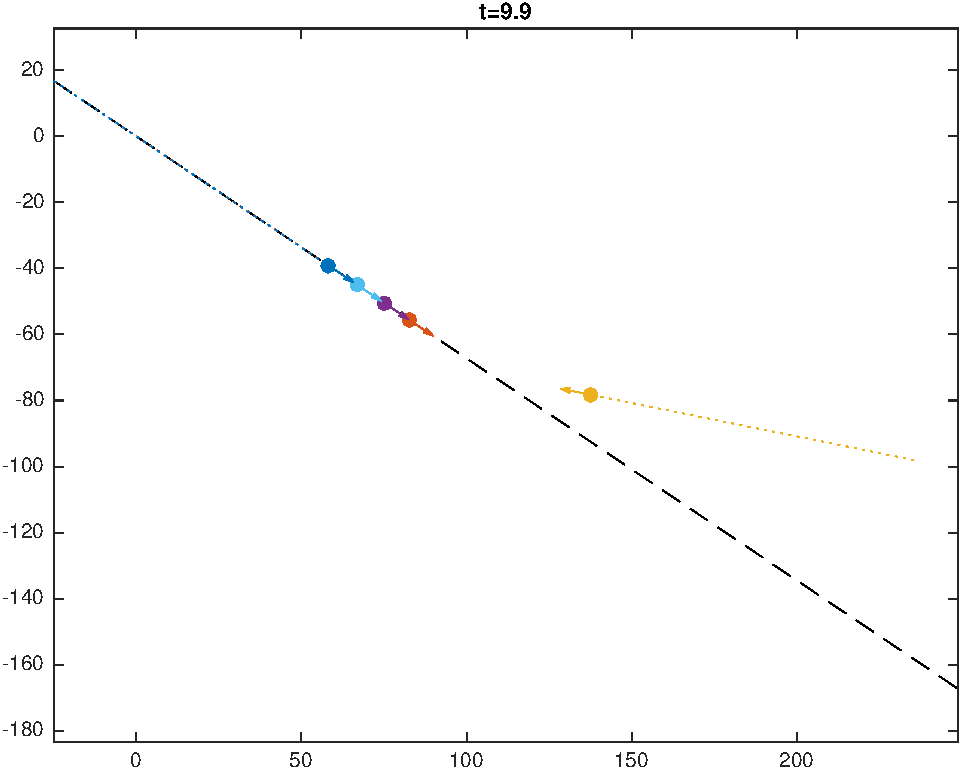
\includegraphics[width=\textwidth]{fig/in_100}
        \caption{100}
    \end{subfigure}
    \begin{subfigure}{0.23\textwidth} \label{subfig:in_120}
        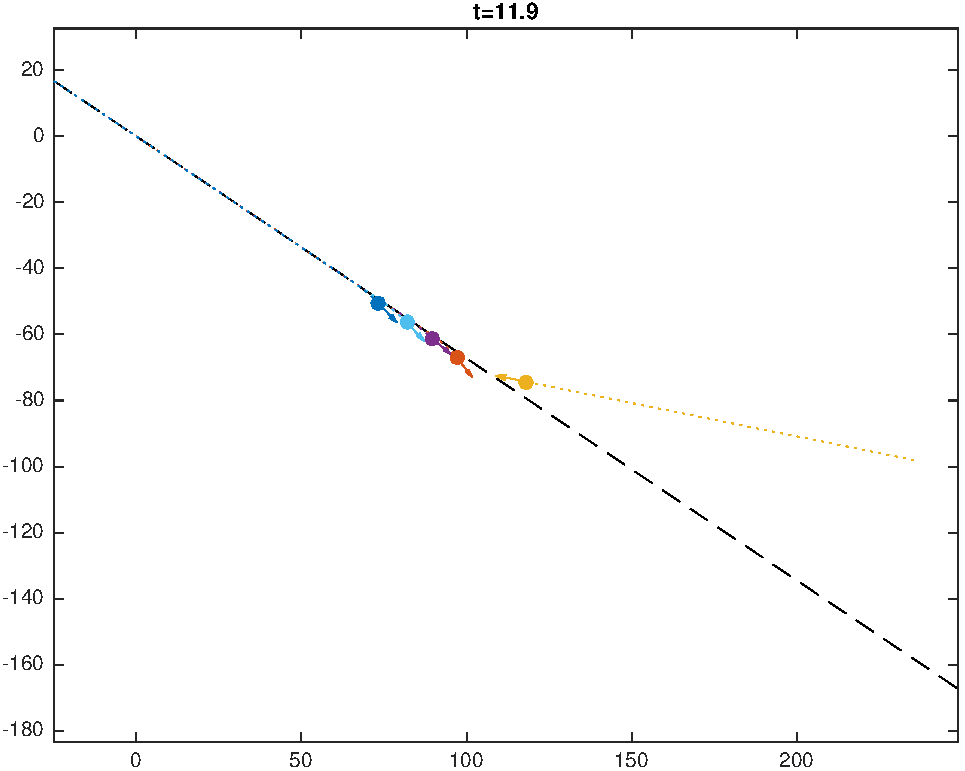
\includegraphics[width=\textwidth]{fig/in_120}
        \caption{120}
    \end{subfigure}

    \begin{subfigure}{0.23\textwidth} \label{subfig:in_140}
        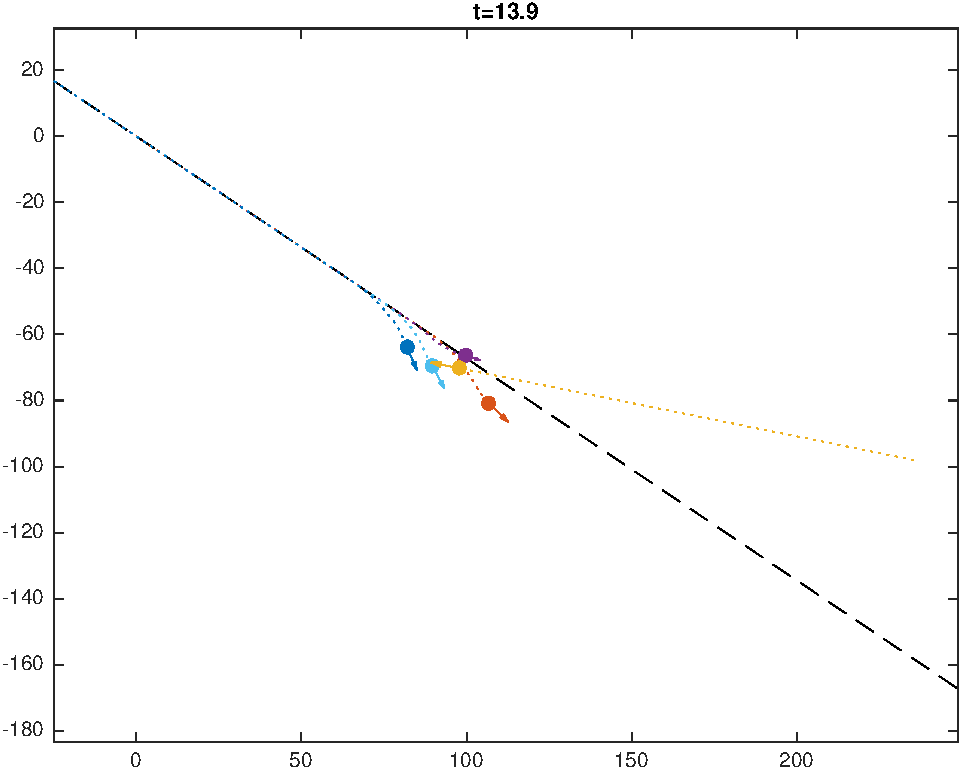
\includegraphics[width=\textwidth]{fig/in_140}
        \caption{140}
    \end{subfigure}
    \begin{subfigure}{0.23\textwidth} \label{subfig:in_200}
        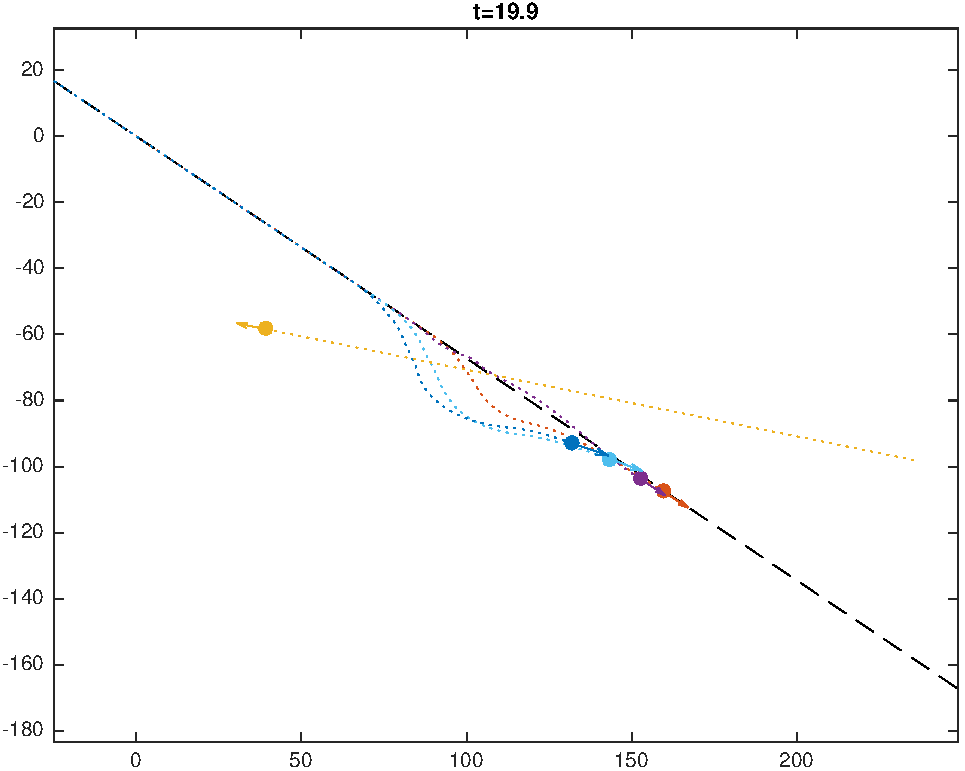
\includegraphics[width=\textwidth]{fig/in_200}
        \caption{200}
    \end{subfigure}   
    \caption{intruder}    
\end{figure}

\subsubsection{Changing highways}

\begin{figure} \label{fig:ch}
    \centering
    \begin{subfigure}{0.23\textwidth} \label{subfig:ch_83}
        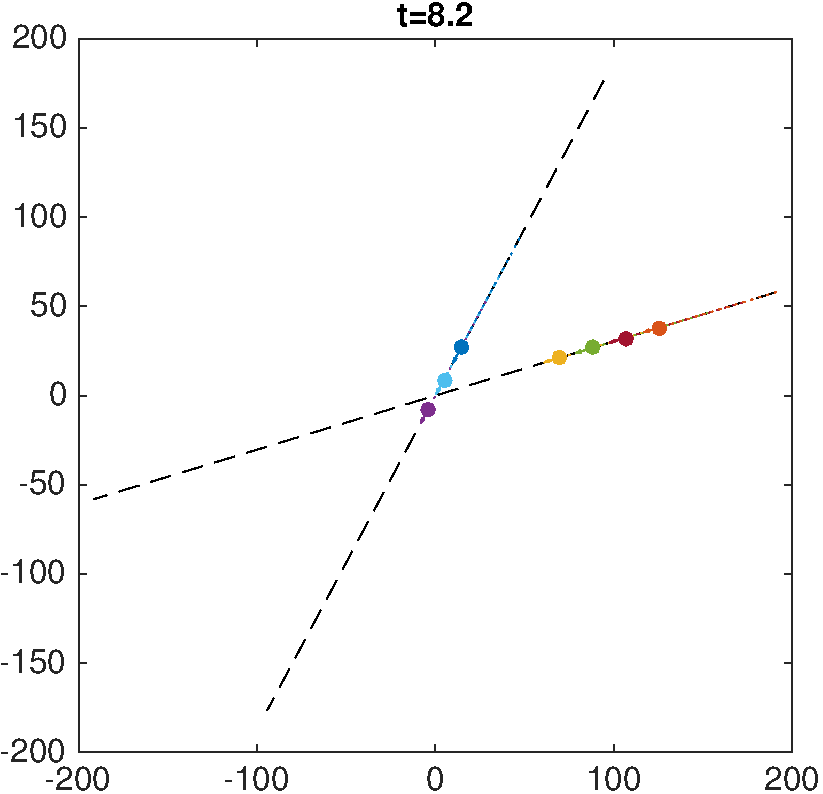
\includegraphics[width=\textwidth]{fig/ch_83}
        \caption{83}
    \end{subfigure}
    \begin{subfigure}{0.23\textwidth} \label{subfig:ch_124}
        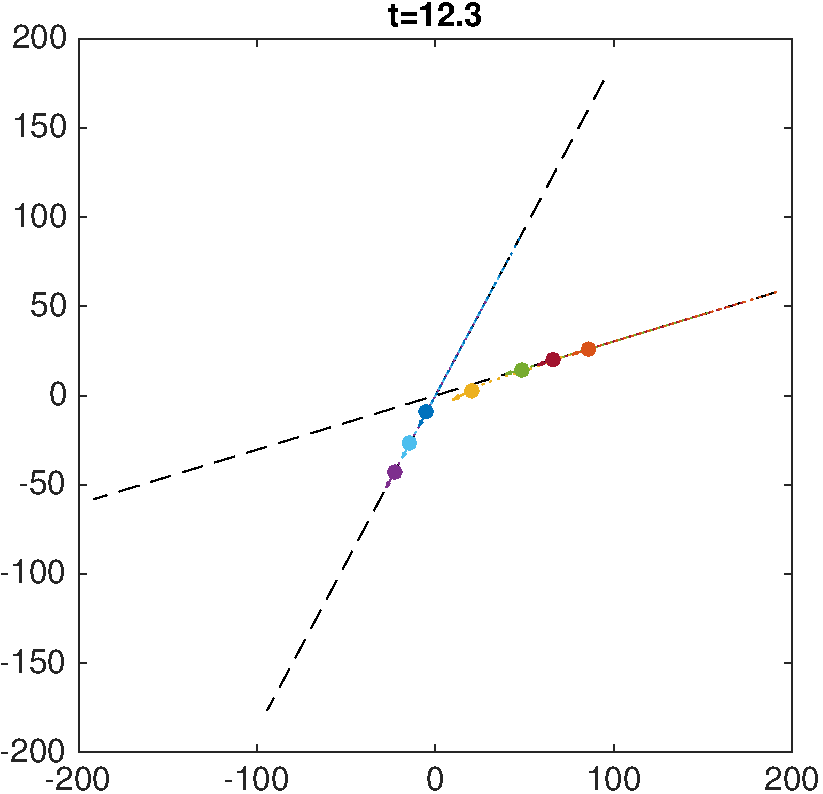
\includegraphics[width=\textwidth]{fig/ch_124}
        \caption{124}
    \end{subfigure}

    \begin{subfigure}{0.23\textwidth} \label{subfig:ch_170}
        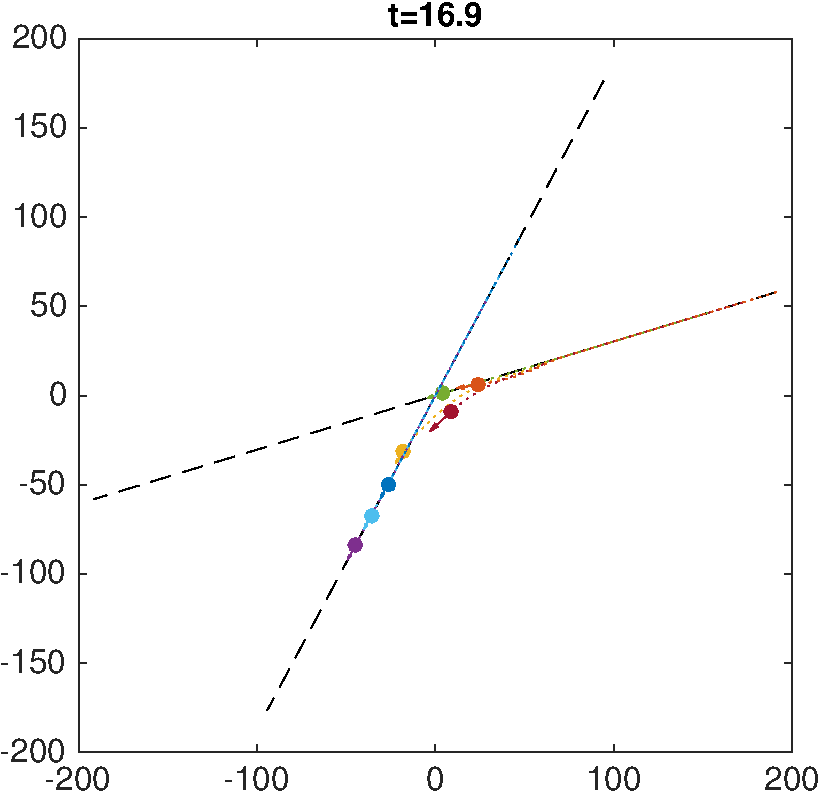
\includegraphics[width=\textwidth]{fig/ch_170}
        \caption{170}
    \end{subfigure}
    \begin{subfigure}{0.23\textwidth} \label{subfig:ch_231}
        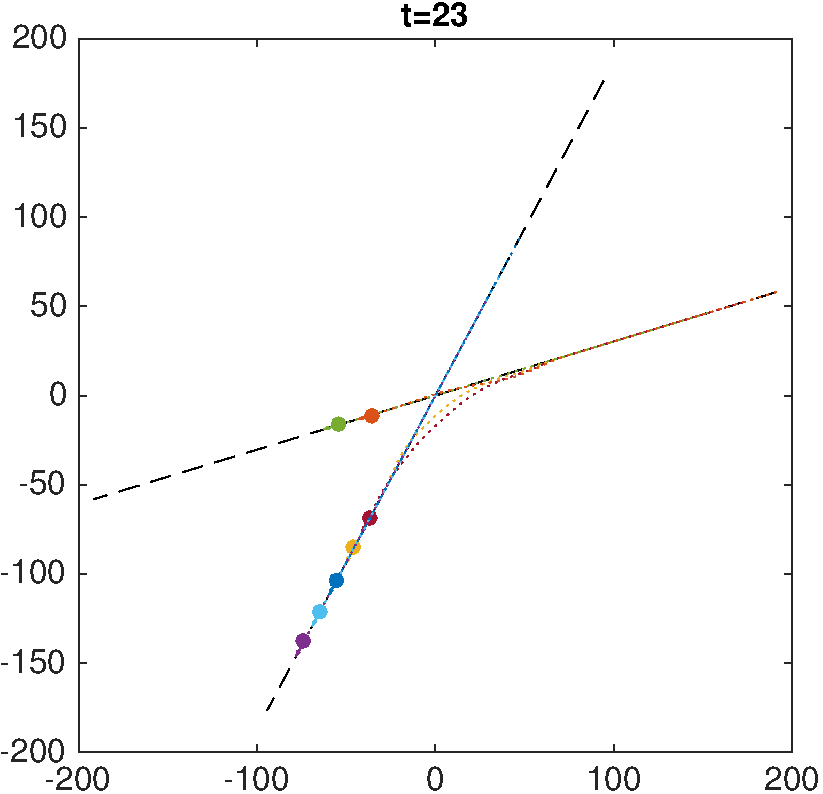
\includegraphics[width=\textwidth]{fig/ch_231}
        \caption{231}
    \end{subfigure}   
    \caption{change highways}    
\end{figure}
